\pdfminorversion=4
\documentclass[aspectratio=169]{beamer}

\mode<presentation>
{
  \usetheme{default}
  \usecolortheme{default}
  \usefonttheme{default}
  \setbeamertemplate{navigation symbols}{}
  \setbeamertemplate{caption}[numbered]
  \setbeamertemplate{footline}[frame number]  % or "page number"
  \setbeamercolor{frametitle}{fg=white}
  \setbeamercolor{footline}{fg=black}
} 

\usepackage[english]{babel}
\usepackage{inputenc}
\usepackage{tikz}
\usepackage{courier}
\usepackage{array}
\usepackage{bold-extra}
\usepackage{minted}
\usepackage[thicklines]{cancel}
\usepackage{fancyvrb}
\usepackage[normalem]{ulem}

\xdefinecolor{dianablue}{rgb}{0.18,0.24,0.31}
\xdefinecolor{darkblue}{rgb}{0.1,0.1,0.7}
\xdefinecolor{darkgreen}{rgb}{0,0.5,0}
\xdefinecolor{darkgrey}{rgb}{0.35,0.35,0.35}
\xdefinecolor{darkorange}{rgb}{0.8,0.5,0}
\xdefinecolor{darkred}{rgb}{0.7,0,0}
\definecolor{darkgreen}{rgb}{0,0.6,0}
\definecolor{mauve}{rgb}{0.58,0,0.82}

\title[2023-11-06-juliahep-physicists]{Engaging the HEP community in Julia}
\author{Jim Pivarski}
\institute{Princeton University -- IRIS-HEP}
\date{November 6, 2023}

\usetikzlibrary{shapes.callouts}

\begin{document}

\logo{\pgfputat{\pgfxy(0.11, 7.4)}{\pgfbox[right,base]{\tikz{\filldraw[fill=dianablue, draw=none] (0 cm, 0 cm) rectangle (50 cm, 1 cm);}\mbox{\hspace{-8 cm}\includegraphics[height=1 cm]{princeton-logo-long.png}\hspace{0.1 cm}\raisebox{0.1 cm}{\includegraphics[height=0.8 cm]{iris-hep-logo-long.png}}\hspace{0.1 cm}}}}}

\begin{frame}
  \titlepage
\end{frame}

\logo{\pgfputat{\pgfxy(0.11, 7.4)}{\pgfbox[right,base]{\tikz{\filldraw[fill=dianablue, draw=none] (0 cm, 0 cm) rectangle (50 cm, 1 cm);}\mbox{\hspace{-8 cm}\includegraphics[height=1 cm]{princeton-logo.png}\hspace{0.1 cm}\raisebox{0.1 cm}{\includegraphics[height=0.8 cm]{iris-hep-logo.png}}\hspace{0.1 cm}}}}}

% Uncomment these lines for an automatically generated outline.
%\begin{frame}{Outline}
%  \tableofcontents
%\end{frame}

% START START START START START START START START START START START START START

\begin{frame}{\mbox{ }}
\LARGE
\begin{center}
\textcolor{darkblue}{Let's start with some numbers\ldots}
\end{center}
\end{frame}

\begin{frame}{State of language use by particle physicists as of last Friday}
\vspace{0.2 cm}
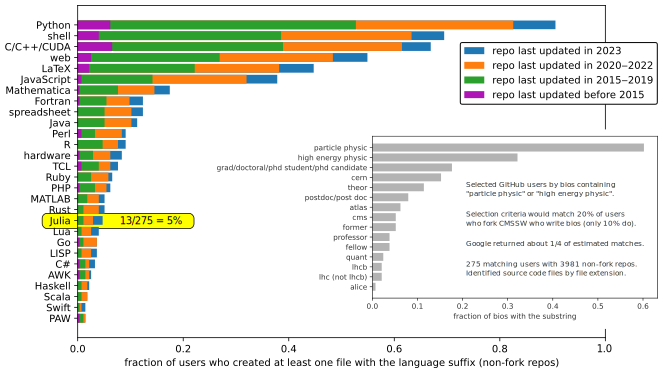
\includegraphics[width=\linewidth]{physicist-languages-presentation.pdf}
\end{frame}

%% "Julia" in Materials, up to a year ago (starting January 2022): 431

%% Removed because author's name is Julia:
%% (+ 1 2 1 1 2 1 1 1 1 6 7 7 7 8 8 7 7 7 7 7 6 7 7 8 8 7 7 8 2 2 4 9 8 8 7 4)
%% 191
%% Documents that reference Julia as a human name:
%% (+ 1 1 1 1 1 1 1 1 1 1 1 1 1 1 1 1 1 1 1 1 1 1 1 1 1 1 1 1 1 1 1 1 1 1 1 1 1 1 1 1 1 1 1 1 1 1 1 1 1 1 1 1 1 1 1 1 1 1 1 1 1 1 1 1 1 1 1 1 1 1 1 1 1 1 1 1 1 1 1 1 1 1 1 1 1 1 1 1 1 1 1 1 1 1 1 1 1 1 1 1 1 1 1 1 1 1 1 1 1 1 1 1 1 1 1 1 1 1 1 1 1 1 1 1 1 1 1 1 1 1 1 1 1)
%% 133
%% Documents that reference Julia the programming language:
%% (+ 1 1 1 1 1 1 1 1 1 1 1 1 1 1 1 1 1 1 1 1 1 1 1 1 1 1 1 1 1 1 1 1 1 1 1 1 1 1 1 1 1 1 1 1 1 1 1 1 1 1 1 1 1 1 1 1 1 1 1 1 1 1 1)
%% 63
%% (1 reference to JULIA (Job to Unveil LEP Interactions in Aleph), 1985-1989)
%% Documents that have no match to "Julia":
%% 1
%% Meaning of "Julia" is other or not clear:
%% 1 1 1

%% "Rust" in Materials, up to a year ago (starting January 2022):

%% Documents that refer to oxidized metal:
%% (+ 1 1 1 1 1 1 1 1 1 1)
%% 10
%% Documents that refer to Rust the programming language:
%% (+ 1 1 1 1 1 1 1 1 1 1 1 1)
%% 12
%% Other/unclear:
%% 1 1 1 

%% "Lua" in Materials, up to a year ago (starting January 2022):

%% Documents that refer to the LHC User's Association:
%% 1 1 1 1

%% Documents that refer to Lua the programming language:
%% 1 (used in SIMION electric field and charge particle simulator)

%% Other/unclear:
%% 1 1 1 1 

\begin{frame}{But physicists are more interested in Julia than, say, Rust or Lua}
\vspace{0.5 cm}
Among ``Materials'' (PDFs and TXTs) in CERN's Indico search since January 2022,

\vspace{0.25 cm}
\begin{description}
\item[\textcolor{darkorange}{\bf 63}] \textcolor{darkorange}{\bf refer to Julia the programming language}
\item[324] refer to people named Julia
\item[4] other/unclear
\end{description}

\begin{description}
\item[\textcolor{darkorange}{\bf 12}] \textcolor{darkorange}{\bf refer to Rust the programming language}

(7 of those same documents also refer to Julia)
\item[10] refer to oxidized metal
\item[3] other/unclear
\end{description}

\begin{description}
\item[\textcolor{darkorange}{\bf 1}] \textcolor{darkorange}{\bf refers to Lua the programming language}

(it's used to configure the SIMION charged particle simulator)
\item[4] refer to the LHC User's Association
\item[4] other/unclear
\end{description}
\end{frame}

%% Julia in CHEP 2023: 3 titles and 4 abstracts
%% 1 1 1 1 

%% Python in CHEP 2023: 1 title and 35 abstracts
%% 1 1 1 1 1 1 1 1 1 1 1 1 1 1 1 1 1 1 1 1 1 1 1 1 1 1 1 1 1 1 1 1 1 1 1 

%% Julia in ACAT 2022: 1 title and 1 abstract
%% Binned histogram fitting for Bayesian inference via Automatic Differentiation in JuliaLang

%% Python in ACAT 2022: 3 titles and 24 abstracts

\begin{frame}{Similarly, it is increasingly a focus on ACAT and CHEP}
\vspace{0.5 cm}

\textcolor{darkblue}{\Large\bf ACAT 2022:}
\begin{itemize}
\item Julia: 1 title and 1 abstract
\item Python: 3 titles and 24 abstracts
\end{itemize}

\vspace{0.5 cm}
\textcolor{darkblue}{\Large\bf CHEP 2023:}
\begin{itemize}
\item Julia: 3 titles and 4 abstracts
\item Python: 1 title and 35 abstracts
\end{itemize}

\vspace{0.5 cm}
Only other programming languages mentioned: C++ (frequently) and Java (2 times).
\end{frame}

\begin{frame}{And, it's the only language-based HSF group other than PyHEP}
\vspace{0.05 cm}
\begin{center}
\includegraphics[width=0.72\linewidth]{juliahep-website.png}
\end{center}
\end{frame}

\begin{frame}{\mbox{ }}
\vspace{0.5 cm}
\LARGE
\begin{center}
\textcolor{darkblue}{Julia is not yet ``adopted'' in HEP, but it is getting more attention than any other rival to C++ and Python.}
\end{center}

\vspace{1 cm}
\begin{center}
\uncover<2->{\textcolor{darkblue}{From here, it could continue to rise in prominence \\ or end up passing as a fad. {\it This is a critical time.}}}
\end{center}
\end{frame}

\begin{frame}{\mbox{ }}
\large
\vspace{0.5 cm}
\textcolor{darkblue}{\Large As we've seen, Julia is a perfect fit for HEP, technologically.}

\vspace{0.5 cm}
\begin{itemize}\setlength{\itemsep}{0.25 cm}
\item<2-> It allows for an exploratory phase, in which the data analyst focuses on {\it what} to compute, rather than how it will be accelerated.
\item<3-> It allows the exploratory code to be tweaked to scale up to large datasets.
\end{itemize}

\vspace{0.5 cm}
\uncover<4->{There is a {\it gradual path} from brainstorming to optimized code, not a rewrite.}
\end{frame}

\begin{frame}{However\ldots}
\vspace{0.5 cm}
\large
\begin{center}
This argument focuses on Julia as a solution to the two-language problem, but we can't go from two languages to one language without going through three.
\end{center}

\vspace{0.25 cm}
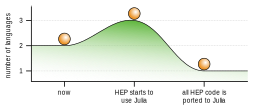
\includegraphics[width=\linewidth]{number-of-languages.pdf}
\end{frame}

\begin{frame}{\sout{``If you build it, they will come.''}}
%% \vspace{-1.55 cm}
%% \hspace{6.5 cm}\includegraphics[height=1 cm]{field-of-dreams.jpg}
%% \vspace{1 cm}

\Large
\vspace{0.6 cm}
Preparing a complete stack of HEP tools in Julia will help adoption, but it will not eliminate the interim 3-language period.

\vspace{0.95 cm}
\uncover<2->{There will not be any clean break in which everyone is ready to set aside their old tools and take up new ones.}

\large
\vspace{0.95 cm}
\uncover<3->{\textcolor{darkgrey}{(The closest approximation to that in HEP was the Fortran $\to$ C++ transition, which was mandated top-down and lost a generation of HEP programmers.)}}
\end{frame}

\begin{frame}{\mbox{ }}
\vspace{0.5 cm}
\LARGE
\begin{center}
\textcolor{darkblue}{We need to give users {\it short-term reasons} to add Julia \\ as a second or third language in their analysis work.}
\end{center}

\vspace{1 cm}
\large
\begin{center}
\uncover<2->{(``You'll be able to replace all your Python and C++'' is a long-term reason.)}
\end{center}
\end{frame}

\begin{frame}{Awkward Array and Julia}
\vspace{0.2 cm}
\only<1>{\includegraphics[width=\linewidth]{awkward-array-website.png}}\only<2>{\includegraphics[width=\linewidth]{awkward-array-jl-website.png}}
\end{frame}

\begin{frame}{This is what I was proposing in 2021}
\vspace{0.1 cm}
\begin{center}
\includegraphics[width=0.88\linewidth]{juliahep-mini-workshop-2021.png}
\end{center}
\end{frame}

\begin{frame}{Awkward Array has other JIT-compiled backends}
\vspace{0.5 cm}
\large
\begin{itemize}\setlength{\itemsep}{0.5 cm}
\item<1-> Numba: \mintinline{python}{ak.Array}s can be arguments and return values of \mintinline{python}{@nb.njit}-compiled functions.
\item<2-> Numba-CUDA: \mintinline{python}{@nb.cuda.njit([extensions=ak.numba.cuda])}.
\item<3-> ROOT RDataFrame: \mintinline{python}{ak.to_rdataframe}/\mintinline{python}{ak.from_rdataframe}.
\item<4-> cppyy: \mintinline{python}{ak.Array}s can be arguments and return values of functions defined by \mintinline{python}{cppyy.cppdef} (pass \mintinline{python}{ak.Array.cpp_type} as its C++ type).
\item<5-> And now Julia.
\end{itemize}
\end{frame}

\begin{frame}{But AwkwardArray.jl isn't like the other backends}
\large
\vspace{0.3 cm}
In both Numba and C++, we define

\vspace{0.25 cm}
\begin{itemize}\setlength{\itemsep}{0.25 cm}
\item<1-> a Python \mintinline{python}{Lookup} object to hold a reference to the \mintinline{python}{ak.Array}, preventing it from going out of scope, and to present its tree-navigation metadata in a raw-byte format, and
\item<1-> a Numba or C++ \mintinline{python}{ArrayView} object that points to a position in the structure, JIT-compiled to behave differently for each tree-node type.
\item<2-> \textcolor{darkblue}{Numba and C++ do not own the array! It's a borrowed reference!}
\end{itemize}

\vspace{0.5 cm}
\uncover<3->{In Julia, we define}

\vspace{0.25 cm}
\begin{itemize}\setlength{\itemsep}{0.25 cm}
\item<3-> the whole layout tree in native Julia structures, and convert.
\item<4-> \textcolor{darkblue}{Julia can own the array!}
\end{itemize}
\end{frame}

\begin{frame}{Python and Julia Awkward Arrays are symmetric, others are not}
\vspace{0.3 cm}

\begin{center}
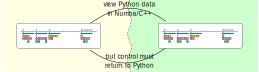
\includegraphics[width=0.9\linewidth]{backends-usage-patterns.pdf}
\end{center}

\vspace{0.1 cm}
\begin{center}
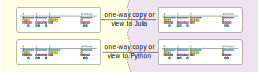
\includegraphics[width=0.9\linewidth]{backends-usage-patterns-2.pdf}
\end{center}
\end{frame}

\begin{frame}{Rationales}
\large
\vspace{0.3 cm}

\begin{itemize}\setlength{\itemsep}{0.5 cm}
\item In Numba, especially Numba-CUDA, only unowned views make sense.

Control {\it will} return to Python.

\item In RDataFrames created from Python, control will return to Python.

We might need to reconsider this if we need to enable \mintinline{c++}{RDataFrame::Snapshot} or distributed RDataFrames.

\item Views make sense for cppyy functions that will deconstruct the \mintinline{python}{ak.Array} before sending it on to other C++ libraries. If Awkward Arrays are to have a life in C++ beyond cppyy, they'll need to be reimplemented as in Julia.

\item In Julia, Awkward Arrays may be passed to other libraries as an opaque \mintinline{julia}{Any}, \mintinline{julia}{AbstractArray}, or a transparent \mintinline{julia}{AwkwardArray.Content}.
\end{itemize}
\end{frame}

\begin{frame}{\mbox{ }}
\vspace{1 cm}
\LARGE
\begin{center}
\textcolor{darkblue}{This also opens the door to UnROOT.jl becoming a drop-in replacement for Uproot in Python workflows.}
\end{center}

\vspace{1 cm}
\begin{center}
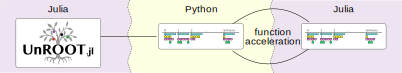
\includegraphics[width=0.9\linewidth]{backends-usage-patterns-3.pdf}
\end{center}
\end{frame}

\begin{frame}{Discussed at PyHEP.dev}
\vspace{0.35 cm}
\begin{center}
\includegraphics[width=\linewidth]{instead-of-uproot-cpp.png}
\end{center}
\end{frame}

\begin{frame}{Technical benefits of AwkwardArray.jl over Python}
\large
\vspace{0.3 cm}
\begin{columns}
\column{1.05\linewidth}

\begin{description}\setlength{\itemsep}{0.5 cm}
\item<1->[\bf Composability:] All buffers in a \mintinline{julia}{AwkwardArray.Content} tree are \mintinline{julia}{AbstractVector}, so it should be easy to swap in special features, like GPU-resident arrays, autodiff, units, etc.

\vspace{0.25 cm}
\uncover<2->{\normalsize In Python, our ``nplike'' backends are complicated by the fact that we have to use array-oriented functions, which is a larger API, and not exactly the same among NumPy, CuPy, JAX, etc. Each new backend needs a shim.}

\item<3->[\bf Unification:] Since \mintinline{julia}{push!} and \mintinline{julia}{append!} are implemented on \mintinline{julia}{AbstractVector}, the functionality of \mintinline{python}{LayoutBuilder} (append-only array) and \mintinline{python}{ak.Array} (read-only array) are unified in the same object.

\vspace{0.25 cm}
\uncover<4->{\normalsize In Python, these need to be two different objects because \mintinline{python}{LayoutBuilder} is only useful in Numba/C++, where arrays are view-only.}
\end{description}
\end{columns}
\end{frame}

\begin{frame}[fragile]{Some examples of AwkwardArray.jl}
\small
\vspace{0.25 cm}
\begin{minted}{julia}
using AwkwardArray
using AwkwardArray: Index64, ListOffsetArray, PrimitiveArray

array = ListOffsetArray{Index64,PrimitiveArray{Float64}}()
push!(array, [1.1, 2.2, 3.3])
push!(array, [4.4])
append!(array, [[5.5, 6.6], [7.7, 8.8, 9.9]])

total = 0.0
for list in array
    for item in list
        total += item
    end
end

vector::Vector{Vector{Float64}} = AwkwardArray.to_vector(array)
array2 = AwkwardArray.from_iter(vector)
\end{minted}
\end{frame}

\begin{frame}{Needs to be connected to Python and ``play well'' with Julia}
\vspace{0.1 cm}
\begin{center}
\includegraphics[width=0.82\linewidth]{issue-5.png}
\end{center}
\end{frame}

\begin{frame}{Don't miss Yana's talk!}
\vspace{0.5 cm}
\includegraphics[width=\linewidth]{ianna-lightning-talk.png}
\end{frame}

\begin{frame}{\mbox{ }}
\vspace{0.5 cm}
\LARGE
\begin{center}
\textcolor{darkblue}{Open question: how does package management \\ work in a Python + Julia environment?}
\end{center}

\vspace{1 cm}
\begin{center}
\uncover<2->{\textcolor{darkblue}{Is there a way to control PyCall/PyJulia's \\ cross-language dependencies with conda?}}
\end{center}
\end{frame}

\begin{frame}{Conclusions}
\vspace{0.5 cm}
\LARGE
\begin{center}
\textcolor{darkblue}{We need stronger connections between HEP analysis tools in Python and HEP analysis tools in Julia.}
\end{center}

\large
\vspace{0.5 cm}
\begin{itemize}\setlength{\itemsep}{0.2 cm}
\item StatsBase.Histogram/FHist.jl generalization that is interchangeable with scikit-hep/boost-histogram, scikit-hep/hist?
\item LorentzVectors.jl or LorentzVectorHEP.jl: interop with scikit-hep/vector?
\item Corpuscles.jl: share data with scikit-hep/particle?
\item IMinuit.jl $\surd$
\item zfit, pyhf, cabinetry, etc.?
\end{itemize}

\normalsize
\vspace{0.5 cm}
\textcolor{darkblue}{Encourage Python users to use Julia {\it with} their Python code! (They won't, otherwise.)}
\end{frame}

\end{document}
